\newpage
\subsubsection{PowerEgg X}
\begin{wrapfigure}{r}{0.3\textwidth}
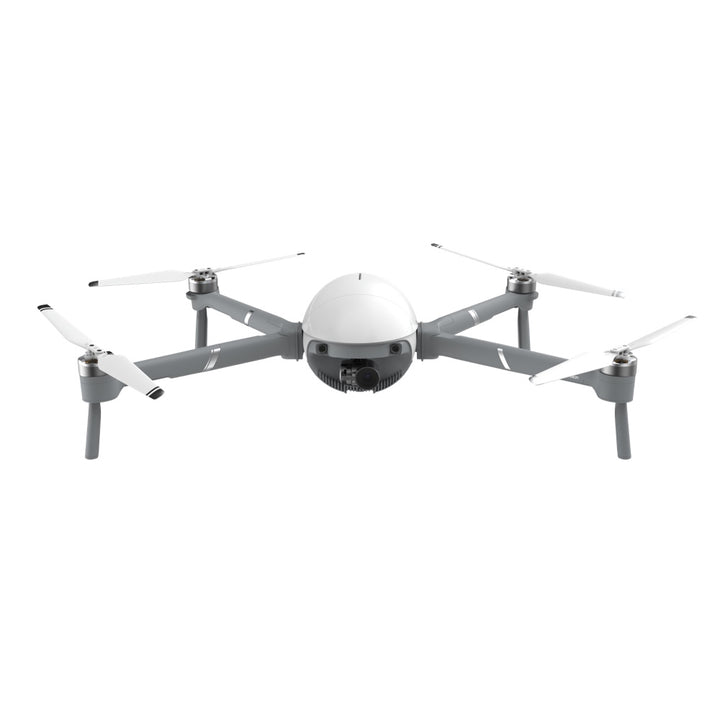
\includegraphics[width=1\linewidth]{uav/models/31_powereggx.jpg}
\caption{PowerEgg X}
\end{wrapfigure}
The PowerEgg X \cite{powereggx} is PowerVision's aerial drone, promoted as a multi-function AI camera.

\paragraph{Payload capacity}\mbox{Score: 0} \\
The payload capacity of the PowerEgg X is not presented on the website and not known from other sources.

\paragraph{Mounting clearance}\mbox{Score: 1.0} \\
The PowerEgg X is a medium sized drone. While it doesn't have special mounting holes, it does have enough clearance on its four horizontal bars

\paragraph{Navigation/Routing}\mbox{Score: 0} \\
While the PowerEgg X does have an app, it doesn't have the ability to set waypoints. Instead, it focuses more on the photography aspects of the drone.

\paragraph{Flight time}\mbox{Score: 1.5} \\
The flight time of the PowerEgg X is 30 minutes, welll passing the minimum required flight time.

\paragraph{Range}\mbox{Score: 1.5} \\
The maximum radio range is 5.9km, well passing the minimum range

\paragraph{Waterproof}\mbox{Score: 1.0} \\
The PowerEgg X has a waterproof kit on the wizard edition. Looking at the specifications, it can be concluded that the drone is rated for IP64 meaning the drone is dust-tight and can sustain splashes. This just meets the minimum required IP rating.

\paragraph{Landing in water}\mbox{Score: 1.3} \\
The PowerEgg X Wizard Edition can land on water with its removable water landing gears

\paragraph{Maneuverability}\mbox{Score: 1.5} \\
The drone can fly horizontally 18m/s. It will recover itself if it is upside down in the water

\paragraph{Total score:}\mbox{0} \\
Due to the PowerEgg X being focused on photography it doesn't have listed payload capacity or the routing capabilities the project needs.

